\documentclass{ctexart}
\usepackage{graphicx}
\xeCJKsetup{CJKecglue={}}
\begin{document}
我们把HPSP算法应用到自然语言的层次聚类问题。
一方面我们通过这个小例子展示HPSP在社团发现实际数据上的效果,
另一方面语言的分类对印欧语言研究较多,已有完善的标准。 
而对其他具体某一地区方言和少数民族语言研究较少,使用
算法自动聚类对于辅助语言学家在后者发力也有裨益 \cite{nasution2019visualizing}。

我们使用的数据是关于词汇相似率的数据。
词汇相似率是一个百分比,表示两种语言中有相同词意和书写方式的词汇比例
\cite{bella2021database}。
我们从Bella提供的数据中选取了世界66种常用语言,选取的标准是原
数据集中词汇相似率置信程度高且两两间均有相似率的语言。
在我们选取的~66~种语言中,其中一种人造语言(世界语),
两种古典语言(梵语、拉丁语),其余均为现代语言。
在此基础上我们用 HPSP 算法进行聚类,得到了如图~\ref{fig:language_tree}所示的聚类树。
\begin{figure}[!ht]
    \centering
    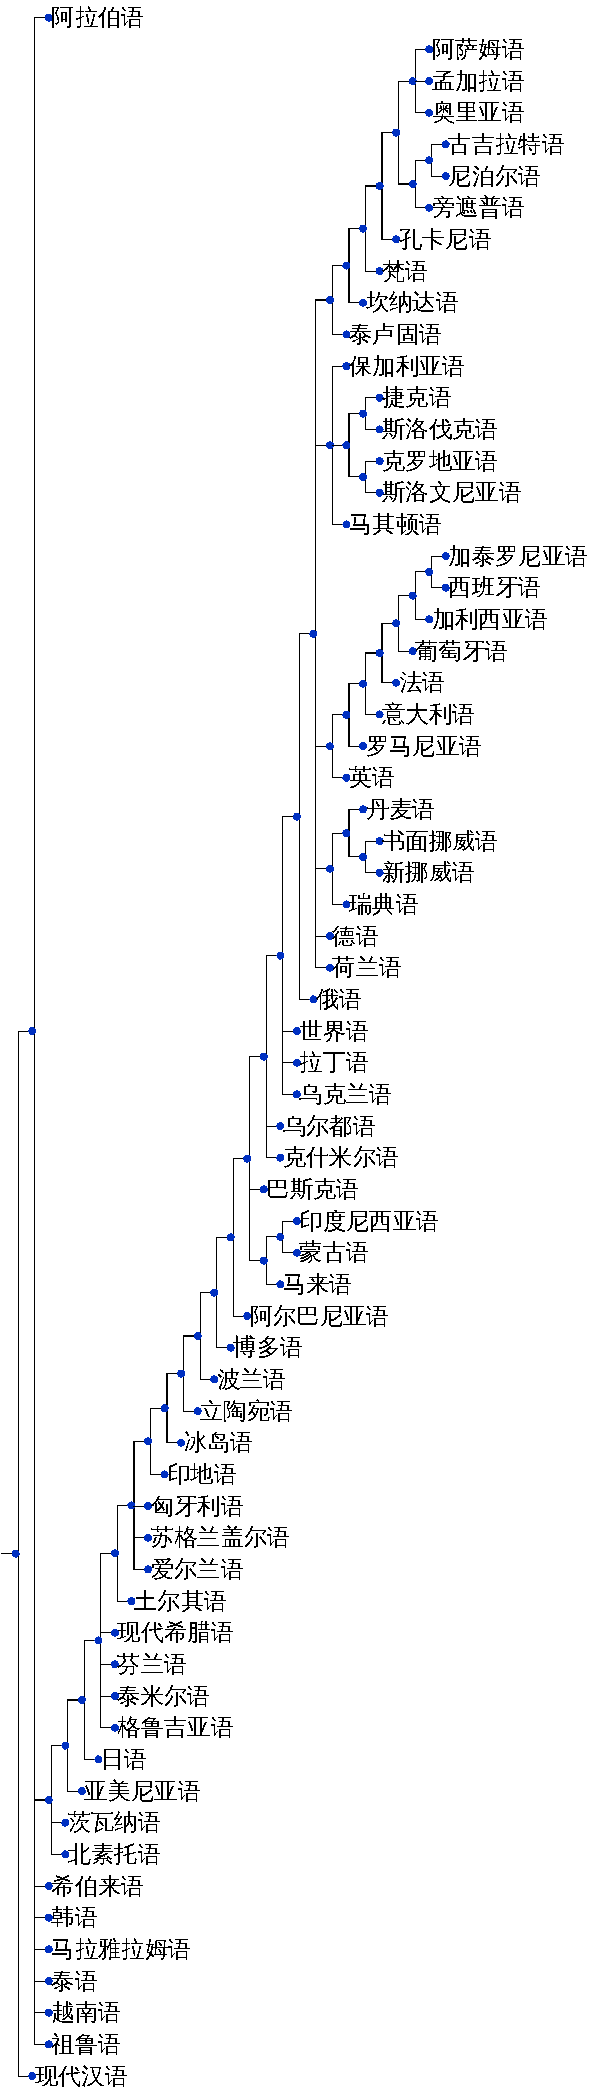
\includegraphics[height=0.9\textheight]{figures/language_tree.pdf}
    \caption{世界常用语言聚类树示意图}\label{fig:language_tree}
\end{figure}

从上图我们可以解读出一些与比较语言学相一致的结论。
首先上图包含了一些在同一国家不同地区使用的语言(西班牙、印度、南非),它们在聚类树中位置较近。
比如西班牙语、加泰罗尼亚语和加利西亚语同属于西班牙,在聚类树中距离很近。
其次从语言进化的角度,具有相同祖先的语言在聚类树中位置较近。比如法语、西班牙语、葡萄牙语、意大利语、
罗马尼亚语同由拉丁语演变而来,
在上图中亦反映出来这五种语言距离很近。

有学者用了普通的聚合聚类的方式对10种常用语言进行聚类 \cite{al2017characterization} 。
我们在这里指出其结果存在一定的不足,比如荷兰语和德语同属于日尔曼语系,在
其获得的聚类树中无法体现,而在我们得到的图中荷兰语和德语的亲近性一目了然。

尽管用算法自动生成的语言聚类树相比语言学家给出的语言进化树仍面临缺少
可解释性和某些方面的准确性,但该方法易拓展到非印欧语系的研究,
为印欧语言和非印欧语言的比较提供了参考。比如从我们的图中可以看到
现代汉语、日语、英语三者的相似度大小,尽管三种语言是属于不同语系。

\bibliographystyle{plain}
\bibliography{ref/refs.bib}

\end{document}
